\documentclass[]{book}
\usepackage{lmodern}
\usepackage{amssymb,amsmath}
\usepackage{ifxetex,ifluatex}
\usepackage{fixltx2e} % provides \textsubscript
\ifnum 0\ifxetex 1\fi\ifluatex 1\fi=0 % if pdftex
  \usepackage[T1]{fontenc}
  \usepackage[utf8]{inputenc}
\else % if luatex or xelatex
  \ifxetex
    \usepackage{mathspec}
  \else
    \usepackage{fontspec}
  \fi
  \defaultfontfeatures{Ligatures=TeX,Scale=MatchLowercase}
\fi
% use upquote if available, for straight quotes in verbatim environments
\IfFileExists{upquote.sty}{\usepackage{upquote}}{}
% use microtype if available
\IfFileExists{microtype.sty}{%
\usepackage{microtype}
\UseMicrotypeSet[protrusion]{basicmath} % disable protrusion for tt fonts
}{}
\usepackage[margin=1in]{geometry}
\usepackage{hyperref}
\hypersetup{unicode=true,
            pdftitle={Data Science With Python},
            pdfauthor={L A Liggett},
            pdfborder={0 0 0},
            breaklinks=true}
\urlstyle{same}  % don't use monospace font for urls
\usepackage{natbib}
\bibliographystyle{apalike}
\usepackage{color}
\usepackage{fancyvrb}
\newcommand{\VerbBar}{|}
\newcommand{\VERB}{\Verb[commandchars=\\\{\}]}
\DefineVerbatimEnvironment{Highlighting}{Verbatim}{commandchars=\\\{\}}
% Add ',fontsize=\small' for more characters per line
\usepackage{framed}
\definecolor{shadecolor}{RGB}{248,248,248}
\newenvironment{Shaded}{\begin{snugshade}}{\end{snugshade}}
\newcommand{\KeywordTok}[1]{\textcolor[rgb]{0.13,0.29,0.53}{\textbf{#1}}}
\newcommand{\DataTypeTok}[1]{\textcolor[rgb]{0.13,0.29,0.53}{#1}}
\newcommand{\DecValTok}[1]{\textcolor[rgb]{0.00,0.00,0.81}{#1}}
\newcommand{\BaseNTok}[1]{\textcolor[rgb]{0.00,0.00,0.81}{#1}}
\newcommand{\FloatTok}[1]{\textcolor[rgb]{0.00,0.00,0.81}{#1}}
\newcommand{\ConstantTok}[1]{\textcolor[rgb]{0.00,0.00,0.00}{#1}}
\newcommand{\CharTok}[1]{\textcolor[rgb]{0.31,0.60,0.02}{#1}}
\newcommand{\SpecialCharTok}[1]{\textcolor[rgb]{0.00,0.00,0.00}{#1}}
\newcommand{\StringTok}[1]{\textcolor[rgb]{0.31,0.60,0.02}{#1}}
\newcommand{\VerbatimStringTok}[1]{\textcolor[rgb]{0.31,0.60,0.02}{#1}}
\newcommand{\SpecialStringTok}[1]{\textcolor[rgb]{0.31,0.60,0.02}{#1}}
\newcommand{\ImportTok}[1]{#1}
\newcommand{\CommentTok}[1]{\textcolor[rgb]{0.56,0.35,0.01}{\textit{#1}}}
\newcommand{\DocumentationTok}[1]{\textcolor[rgb]{0.56,0.35,0.01}{\textbf{\textit{#1}}}}
\newcommand{\AnnotationTok}[1]{\textcolor[rgb]{0.56,0.35,0.01}{\textbf{\textit{#1}}}}
\newcommand{\CommentVarTok}[1]{\textcolor[rgb]{0.56,0.35,0.01}{\textbf{\textit{#1}}}}
\newcommand{\OtherTok}[1]{\textcolor[rgb]{0.56,0.35,0.01}{#1}}
\newcommand{\FunctionTok}[1]{\textcolor[rgb]{0.00,0.00,0.00}{#1}}
\newcommand{\VariableTok}[1]{\textcolor[rgb]{0.00,0.00,0.00}{#1}}
\newcommand{\ControlFlowTok}[1]{\textcolor[rgb]{0.13,0.29,0.53}{\textbf{#1}}}
\newcommand{\OperatorTok}[1]{\textcolor[rgb]{0.81,0.36,0.00}{\textbf{#1}}}
\newcommand{\BuiltInTok}[1]{#1}
\newcommand{\ExtensionTok}[1]{#1}
\newcommand{\PreprocessorTok}[1]{\textcolor[rgb]{0.56,0.35,0.01}{\textit{#1}}}
\newcommand{\AttributeTok}[1]{\textcolor[rgb]{0.77,0.63,0.00}{#1}}
\newcommand{\RegionMarkerTok}[1]{#1}
\newcommand{\InformationTok}[1]{\textcolor[rgb]{0.56,0.35,0.01}{\textbf{\textit{#1}}}}
\newcommand{\WarningTok}[1]{\textcolor[rgb]{0.56,0.35,0.01}{\textbf{\textit{#1}}}}
\newcommand{\AlertTok}[1]{\textcolor[rgb]{0.94,0.16,0.16}{#1}}
\newcommand{\ErrorTok}[1]{\textcolor[rgb]{0.64,0.00,0.00}{\textbf{#1}}}
\newcommand{\NormalTok}[1]{#1}
\usepackage{longtable,booktabs}
\usepackage{graphicx,grffile}
\makeatletter
\def\maxwidth{\ifdim\Gin@nat@width>\linewidth\linewidth\else\Gin@nat@width\fi}
\def\maxheight{\ifdim\Gin@nat@height>\textheight\textheight\else\Gin@nat@height\fi}
\makeatother
% Scale images if necessary, so that they will not overflow the page
% margins by default, and it is still possible to overwrite the defaults
% using explicit options in \includegraphics[width, height, ...]{}
\setkeys{Gin}{width=\maxwidth,height=\maxheight,keepaspectratio}
\IfFileExists{parskip.sty}{%
\usepackage{parskip}
}{% else
\setlength{\parindent}{0pt}
\setlength{\parskip}{6pt plus 2pt minus 1pt}
}
\setlength{\emergencystretch}{3em}  % prevent overfull lines
\providecommand{\tightlist}{%
  \setlength{\itemsep}{0pt}\setlength{\parskip}{0pt}}
\setcounter{secnumdepth}{5}
% Redefines (sub)paragraphs to behave more like sections
\ifx\paragraph\undefined\else
\let\oldparagraph\paragraph
\renewcommand{\paragraph}[1]{\oldparagraph{#1}\mbox{}}
\fi
\ifx\subparagraph\undefined\else
\let\oldsubparagraph\subparagraph
\renewcommand{\subparagraph}[1]{\oldsubparagraph{#1}\mbox{}}
\fi

%%% Use protect on footnotes to avoid problems with footnotes in titles
\let\rmarkdownfootnote\footnote%
\def\footnote{\protect\rmarkdownfootnote}

%%% Change title format to be more compact
\usepackage{titling}

% Create subtitle command for use in maketitle
\newcommand{\subtitle}[1]{
  \posttitle{
    \begin{center}\large#1\end{center}
    }
}

\setlength{\droptitle}{-2em}

  \title{Data Science With Python}
    \pretitle{\vspace{\droptitle}\centering\huge}
  \posttitle{\par}
    \author{L A Liggett}
    \preauthor{\centering\large\emph}
  \postauthor{\par}
      \predate{\centering\large\emph}
  \postdate{\par}
    \date{2019-04-16}

\usepackage{booktabs}
\usepackage{amsthm}
\makeatletter
\def\thm@space@setup{%
  \thm@preskip=8pt plus 2pt minus 4pt
  \thm@postskip=\thm@preskip
}
\makeatother

\begin{document}
\maketitle

{
\setcounter{tocdepth}{1}
\tableofcontents
}
\chapter{Prerequisites}\label{prerequisites}

This is a \emph{sample} book written in \textbf{Markdown}. You can use
anything that Pandoc's Markdown supports, e.g., a math equation
\(a^2 + b^2 = c^2\).

The \textbf{bookdown} package can be installed from CRAN or Github:

\begin{Shaded}
\begin{Highlighting}[]
\KeywordTok{install.packages}\NormalTok{(}\StringTok{"bookdown"}\NormalTok{)}
\CommentTok{# or the development version}
\CommentTok{# devtools::install_github("rstudio/bookdown")}
\end{Highlighting}
\end{Shaded}

Remember each Rmd file contains one and only one chapter, and a chapter
is defined by the first-level heading \texttt{\#}.

To compile this example to PDF, you need XeLaTeX. You are recommended to
install TinyTeX (which includes XeLaTeX):
\url{https://yihui.name/tinytex/}.

\chapter{Introduction}\label{intro}

You can label chapter and section titles using \texttt{\{\#label\}}
after them, e.g., we can reference Chapter \ref{intro}. If you do not
manually label them, there will be automatic labels anyway, e.g.,
Chapter \ref{visualization}.

Figures and tables with captions will be placed in \texttt{figure} and
\texttt{table} environments, respectively.

And this is some other random stuff.

\begin{Shaded}
\begin{Highlighting}[]
\KeywordTok{par}\NormalTok{(}\DataTypeTok{mar =} \KeywordTok{c}\NormalTok{(}\DecValTok{4}\NormalTok{, }\DecValTok{4}\NormalTok{, .}\DecValTok{1}\NormalTok{, .}\DecValTok{1}\NormalTok{))}
\KeywordTok{plot}\NormalTok{(pressure, }\DataTypeTok{type =} \StringTok{'b'}\NormalTok{, }\DataTypeTok{pch =} \DecValTok{19}\NormalTok{)}
\end{Highlighting}
\end{Shaded}

\begin{figure}

{\centering 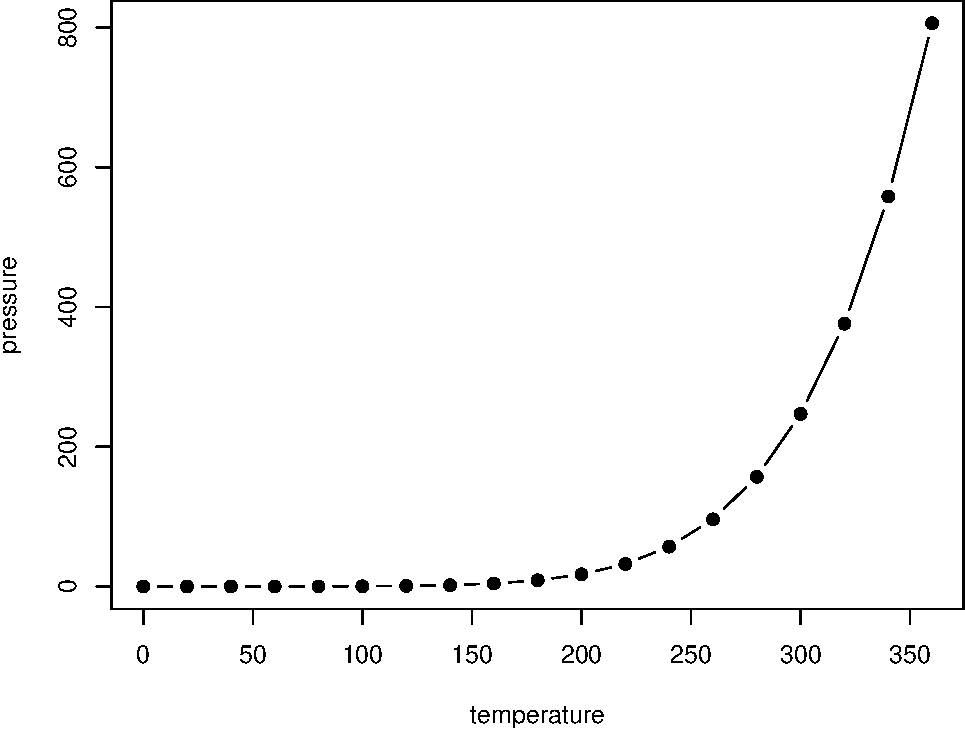
\includegraphics[width=0.8\linewidth]{bookdown-demo_files/figure-latex/nice-fig-1} 

}

\caption{Here is a nice figure!}\label{fig:nice-fig}
\end{figure}

Reference a figure by its code chunk label with the \texttt{fig:}
prefix, e.g., see Figure \ref{fig:nice-fig}. Similarly, you can
reference tables generated from \texttt{knitr::kable()}, e.g., see Table
\ref{tab:nice-tab}.

\begin{Shaded}
\begin{Highlighting}[]
\NormalTok{knitr}\OperatorTok{::}\KeywordTok{kable}\NormalTok{(}
  \KeywordTok{head}\NormalTok{(iris, }\DecValTok{20}\NormalTok{), }\DataTypeTok{caption =} \StringTok{'Here is a nice table!'}\NormalTok{,}
  \DataTypeTok{booktabs =} \OtherTok{TRUE}
\NormalTok{)}
\end{Highlighting}
\end{Shaded}

\begin{table}[t]

\caption{\label{tab:nice-tab}Here is a nice table!}
\centering
\begin{tabular}{rrrrl}
\toprule
Sepal.Length & Sepal.Width & Petal.Length & Petal.Width & Species\\
\midrule
5.1 & 3.5 & 1.4 & 0.2 & setosa\\
4.9 & 3.0 & 1.4 & 0.2 & setosa\\
4.7 & 3.2 & 1.3 & 0.2 & setosa\\
4.6 & 3.1 & 1.5 & 0.2 & setosa\\
5.0 & 3.6 & 1.4 & 0.2 & setosa\\
\addlinespace
5.4 & 3.9 & 1.7 & 0.4 & setosa\\
4.6 & 3.4 & 1.4 & 0.3 & setosa\\
5.0 & 3.4 & 1.5 & 0.2 & setosa\\
4.4 & 2.9 & 1.4 & 0.2 & setosa\\
4.9 & 3.1 & 1.5 & 0.1 & setosa\\
\addlinespace
5.4 & 3.7 & 1.5 & 0.2 & setosa\\
4.8 & 3.4 & 1.6 & 0.2 & setosa\\
4.8 & 3.0 & 1.4 & 0.1 & setosa\\
4.3 & 3.0 & 1.1 & 0.1 & setosa\\
5.8 & 4.0 & 1.2 & 0.2 & setosa\\
\addlinespace
5.7 & 4.4 & 1.5 & 0.4 & setosa\\
5.4 & 3.9 & 1.3 & 0.4 & setosa\\
5.1 & 3.5 & 1.4 & 0.3 & setosa\\
5.7 & 3.8 & 1.7 & 0.3 & setosa\\
5.1 & 3.8 & 1.5 & 0.3 & setosa\\
\bottomrule
\end{tabular}
\end{table}

\begin{Shaded}
\begin{Highlighting}[]
\NormalTok{knitr}\OperatorTok{::}\KeywordTok{include_graphics}\NormalTok{(}\KeywordTok{rep}\NormalTok{(}\StringTok{"knit-logo.png"}\NormalTok{, }\DecValTok{3}\NormalTok{))}
\end{Highlighting}
\end{Shaded}

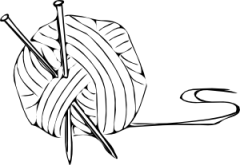
\includegraphics{knit-logo.png} 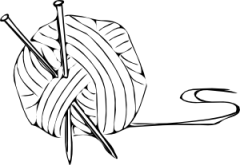
\includegraphics{knit-logo.png}
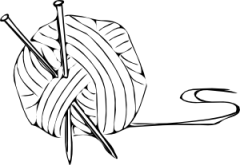
\includegraphics{knit-logo.png}

\begin{Shaded}
\begin{Highlighting}[]
\NormalTok{knitr}\OperatorTok{::}\KeywordTok{include_app}\NormalTok{(}\StringTok{"https://yihui.shinyapps.io/miniUI/"}\NormalTok{, }
                     \DataTypeTok{height =} \StringTok{"600px"}\NormalTok{)}
\end{Highlighting}
\end{Shaded}

\begin{Shaded}
\begin{Highlighting}[]
\ImportTok{import}\NormalTok{ pandas }\ImportTok{as}\NormalTok{ pd}
\NormalTok{x }\OperatorTok{=} \StringTok{'hello, python world!'}
\BuiltInTok{print}\NormalTok{(x.split(}\StringTok{' '}\NormalTok{))}
\end{Highlighting}
\end{Shaded}

\begin{verbatim}
## ['hello,', 'python', 'world!']
\end{verbatim}

You can write citations, too. For example, we are using the
\textbf{bookdown} package \citep{R-bookdown} in this sample book, which
was built on top of R Markdown and \textbf{knitr} \citep{xie2015}.

\chapter{JupyterLab}\label{jupyter}

Here is a simple template that I use that controls a couple useful
things when starting a new notebook.

\begin{Shaded}
\begin{Highlighting}[]
\ImportTok{import}\NormalTok{ sys}
\NormalTok{sys.path.append(}\StringTok{'../util'}\NormalTok{)}

\OperatorTok\NormalTok{autoreload }\DecValTok{2}

\ImportTok{from}\NormalTok{ util }\ImportTok{import} \OperatorTok{*}
\ImportTok{import}\NormalTok{ numpy }\ImportTok{as}\NormalTok{ np                  }
\ImportTok{import}\NormalTok{ pandas }\ImportTok{as}\NormalTok{ pd                 }
\ImportTok{from}\NormalTok{ matplotlib }\ImportTok{import}\NormalTok{ pyplot }\ImportTok{as}\NormalTok{ plt}
\ImportTok{import}\NormalTok{ seaborn }\ImportTok{as}\NormalTok{ sns}

\NormalTok{sns.set_palette(}\StringTok{'pastel'}\NormalTok{)}
\NormalTok{sns.set_style(}\StringTok{'ticks'}\NormalTok{)}
\NormalTok{sns.set_context(}\StringTok{'paper'}\NormalTok{, font_scale}\OperatorTok{=}\DecValTok{1}\NormalTok{)}
\end{Highlighting}
\end{Shaded}

It is often convenient to have a notebook automatically refresh the
imported libraries so that they can be modified while working on a
JupyterLab notebook.

\begin{Shaded}
\begin{Highlighting}[]
\OperatorTok\NormalTok{autoreload }\DecValTok{2}
\end{Highlighting}
\end{Shaded}

To allow directory organization, dependcies can be separated into
different directories and imported into a jupyter notebook using the
following import statement.

\begin{Shaded}
\begin{Highlighting}[]
\ImportTok{import}\NormalTok{ sys}
\NormalTok{sys.path.append(}\StringTok{'../util'}\NormalTok{)}
\end{Highlighting}
\end{Shaded}

\chapter{Visualization}\label{visualization}

\section{Colorschemes}\label{colorschemes}

Seaborn Themes Pastel: {[}Blue:`\#a3c6ff', Orange:`\#f7ab60',
Green:`\#60f7a9', Red:`\#fc9d94', Purple:`\#bea3ff', Brown:`\#d1b485',
Pink:`\#f7afdf', Gray:`\#c4c4c4', Yellow:`\#ffffaa', LBlue:`\#baf6ff'{]}
Deep: {[}Green:`\#5baf68'{]}

\section{Matplotlib}\label{matplotlib}

Plotting a heatmap.

\begin{Shaded}
\begin{Highlighting}[]
\ImportTok{import}\NormalTok{ matplotlib.pyplot }\ImportTok{as}\NormalTok{ plt}
\ImportTok{import}\NormalTok{ numpy }\ImportTok{as}\NormalTok{ np}
\NormalTok{a }\OperatorTok{=}\NormalTok{ np.random.random((}\DecValTok{16}\NormalTok{, }\DecValTok{16}\NormalTok{))}
\NormalTok{plt.imshow(a, cmap}\OperatorTok{=}\StringTok{'RdBu'', interpolation='}\NormalTok{nearest}\StringTok{')}
\StringTok{plt.show()}
\end{Highlighting}
\end{Shaded}

Possible heatmap colors are:

\begin{Shaded}
\begin{Highlighting}[]
\NormalTok{Accent, Accent_r, Blues, Blues_r, BrBG, BrBG_r, BuGn, BuGn_r, BuPu, BuPu_r, CMRmap, CMRmap_r, Dark2, Dark2_r, GnBu, GnBu_r, Greens, Greens_r, Greys, Greys_r, OrRd, OrRd_r, Oranges, Oranges_r, PRGn, PRGn_r, Paired, Paired_r, Pastel1, Pastel1_r, Pastel2, Pastel2_r, PiYG, PiYG_r, PuBu, PuBuGn, PuBuGn_r, PuBu_r, PuOr, PuOr_r, PuRd, PuRd_r, Purples, Purples_r, RdBu, RdBu_r, RdGy, RdGy_r, RdPu, RdPu_r, RdYlBu, RdYlBu_r, RdYlGn, RdYlGn_r, Reds, Reds_r, Set1,}
\NormalTok{Set1_r, Set2, Set2_r, Set3, Set3_r, Spectral, Spectral_r, Wistia, Wistia_r, YlGn, YlGnBu, YlGnBu_r, YlGn_r, YlOrBr, YlOrBr_r, YlOrRd, YlOrRd_r, afmhot, afmhot_r, autumn, autumn_r, binary, binary_r, bone, bone_r, brg, brg_r, bwr, bwr_r, cividis, cividis_r, cool, cool_r, coolwarm, coolwarm_r, copper, copper_r, cubehelix, cubehelix_r, flag, flag_r, gist_earth, gist_earth_r, gist_gray, gist_gray_r, gist_heat, gist_heat_r, gist_ncar, gist_ncar_r, gist_rainbow, gist_rainbow_r,}
\NormalTok{gist_stern, gist_stern_r, gist_yarg, gist_yarg_r, gnuplot, gnuplot2, gnuplot2_r, gnuplot_r, gray, gray_r, hot, hot_r, hsv, hsv_r, icefire, icefire_r, inferno, inferno_r, jet, jet_r, magma, magma_r, mako, mako_r, nipy_spectral, nipy_spectral_r, ocean, ocean_r, pink, pink_r, plasma, plasma_r, prism, prism_r, rainbow, rainbow_r, rocket, rocket_r, seismic, seismic_r, spring, spring_r, summer, summer_r, tab10, tab10_r, tab20, tab20_r, tab20b, tab20b_r, tab20c, tab20c_r, terrain, terrain_r,}
\NormalTok{twilight, twilight_r, twilight_shifted, twilight_shifted_r, viridis, viridis_r, vlag, vlag_r, winter, winter_r}
\end{Highlighting}
\end{Shaded}

A simple venn diagram.

\begin{Shaded}
\begin{Highlighting}[]
\ImportTok{from}\NormalTok{ matplotlib_venn }\ImportTok{import}\NormalTok{ venn2}
\NormalTok{venn2(subsets }\OperatorTok{=}\NormalTok{ (}\DecValTok{3}\NormalTok{, }\DecValTok{2}\NormalTok{, }\DecValTok{1}\NormalTok{))}
\end{Highlighting}
\end{Shaded}

A more complicated venn diagram.

\begin{Shaded}
\begin{Highlighting}[]
\ImportTok{from}\NormalTok{ matplotlib }\ImportTok{import}\NormalTok{ pyplot }\ImportTok{as}\NormalTok{ plt}
\ImportTok{import}\NormalTok{ numpy }\ImportTok{as}\NormalTok{ np}
\ImportTok{from}\NormalTok{ matplotlib_venn }\ImportTok{import}\NormalTok{ venn3, venn3_circles}
\NormalTok{plt.figure(figsize}\OperatorTok{=}\NormalTok{(}\DecValTok{4}\NormalTok{,}\DecValTok{4}\NormalTok{))}
\NormalTok{v }\OperatorTok{=}\NormalTok{ venn3(subsets}\OperatorTok{=}\NormalTok{(}\DecValTok{1}\NormalTok{, }\DecValTok{1}\NormalTok{, }\DecValTok{1}\NormalTok{, }\DecValTok{1}\NormalTok{, }\DecValTok{1}\NormalTok{, }\DecValTok{1}\NormalTok{, }\DecValTok{1}\NormalTok{), set_labels }\OperatorTok{=}\NormalTok{ (}\StringTok{'A'}\NormalTok{, }\StringTok{'B'}\NormalTok{, }\StringTok{'C'}\NormalTok{))}
\NormalTok{v.get_patch_by_id(}\StringTok{'100'}\NormalTok{).set_alpha(}\FloatTok{1.0}\NormalTok{)}
\NormalTok{v.get_patch_by_id(}\StringTok{'100'}\NormalTok{).set_color(}\StringTok{'white'}\NormalTok{)}
\NormalTok{v.get_label_by_id(}\StringTok{'100'}\NormalTok{).set_text(}\StringTok{'Unknown'}\NormalTok{)}
\NormalTok{v.get_label_by_id(}\StringTok{'A'}\NormalTok{).set_text(}\StringTok{'Set "A"'}\NormalTok{)}
\NormalTok{c }\OperatorTok{=}\NormalTok{ venn3_circles(subsets}\OperatorTok{=}\NormalTok{(}\DecValTok{1}\NormalTok{, }\DecValTok{1}\NormalTok{, }\DecValTok{1}\NormalTok{, }\DecValTok{1}\NormalTok{, }\DecValTok{1}\NormalTok{, }\DecValTok{1}\NormalTok{, }\DecValTok{1}\NormalTok{), linestyle}\OperatorTok{=}\StringTok{'dotted'}\NormalTok{)}
\NormalTok{c[}\DecValTok{0}\NormalTok{].set_lw(}\FloatTok{1.0}\NormalTok{)}
\NormalTok{c[}\DecValTok{0}\NormalTok{].set_ls(}\StringTok{'dotted'}\NormalTok{)}
\NormalTok{plt.title(}\StringTok{"Sample Venn diagram"}\NormalTok{)}
\NormalTok{plt.annotate(}\StringTok{'Unknown set'}\NormalTok{, xy}\OperatorTok{=}\NormalTok{v.get_label_by_id(}\StringTok{'100'}\NormalTok{).get_position() }\OperatorTok{-}\NormalTok{ np.array([}\DecValTok{0}\NormalTok{, }\FloatTok{0.05}\NormalTok{]), xytext}\OperatorTok{=}\NormalTok{(}\OperatorTok{-}\DecValTok{70}\NormalTok{,}\OperatorTok{-}\DecValTok{70}\NormalTok{),}
\NormalTok{             ha}\OperatorTok{=}\StringTok{'center'}\NormalTok{, textcoords}\OperatorTok{=}\StringTok{'offset points'}\NormalTok{, bbox}\OperatorTok{=}\BuiltInTok{dict}\NormalTok{(boxstyle}\OperatorTok{=}\StringTok{'round,pad=0.5'}\NormalTok{, fc}\OperatorTok{=}\StringTok{'gray'}\NormalTok{, alpha}\OperatorTok{=}\FloatTok{0.1}\NormalTok{),}
\NormalTok{                          arrowprops}\OperatorTok{=}\BuiltInTok{dict}\NormalTok{(arrowstyle}\OperatorTok{=}\StringTok{'->'}\NormalTok{, connectionstyle}\OperatorTok{=}\StringTok{'arc3,rad=0.5'}\NormalTok{,color}\OperatorTok{=}\StringTok{'gray'}\NormalTok{))}
\NormalTok{                          plt.show()}
\end{Highlighting}
\end{Shaded}

\section{Seaborn}\label{seaborn}

Here is a general bar plot that includes some commonly used parameters.

\begin{Shaded}
\begin{Highlighting}[]
\CommentTok{# fits my 22 inch monitor}
\NormalTok{plt.figure(figsize}\OperatorTok{=}\NormalTok{(}\FloatTok{19.17}\NormalTok{,}\FloatTok{11.98}\NormalTok{))}
\CommentTok{# order controls the display order of the samples}
\NormalTok{sns.catplot(x}\OperatorTok{=}\StringTok{"Sample"}\NormalTok{, y}\OperatorTok{=}\StringTok{"Somatic"}\NormalTok{, kind}\OperatorTok{=}\StringTok{"bar"}\NormalTok{, data}\OperatorTok{=}\NormalTok{var_counts, order}\OperatorTok{=}\NormalTok{labels)}\OperatorTok{;}
\CommentTok{# keeps x-axis labels, but eliminates the tick mark}
\NormalTok{plt.tick_params(labelbottom}\OperatorTok{=}\VariableTok{True}\NormalTok{, bottom}\OperatorTok{=}\VariableTok{False}\NormalTok{)}
\CommentTok{# trim off the x-axis}
\NormalTok{sns.despine(offset}\OperatorTok{=}\DecValTok{10}\NormalTok{, trim}\OperatorTok{=}\VariableTok{True}\NormalTok{, bottom}\OperatorTok{=}\VariableTok{True}\NormalTok{)}
\CommentTok{# labels}
\NormalTok{plt.title(}\StringTok{''}\NormalTok{)}
\NormalTok{plt.ylabel(}\StringTok{''}\NormalTok{)}
\NormalTok{plt.xlabel(}\StringTok{''}\NormalTok{)}
\CommentTok{# manual control of xlabels}
\NormalTok{labels }\OperatorTok{=}\NormalTok{ [}\StringTok{'Indiv_1-a'}\NormalTok{,}\StringTok{'Indiv_2'}\NormalTok{,}\StringTok{'Indiv_3'}\NormalTok{,}\StringTok{'Indiv_1-b'}\NormalTok{]}
\CommentTok{# control xtick order}
\NormalTok{plt.xticks(}\BuiltInTok{range}\NormalTok{(}\BuiltInTok{len}\NormalTok{(labels)), labels, rotation}\OperatorTok{=}\DecValTok{45}\NormalTok{)}
\CommentTok{# control the number of x-ticks}
\NormalTok{plt.locator_params(axis}\OperatorTok{=}\StringTok{'x'}\NormalTok{, nbins}\OperatorTok{=}\DecValTok{10}\NormalTok{)}
\CommentTok{# legend positioning}
\NormalTok{plt.legend(loc}\OperatorTok{=}\StringTok{'upper right'}\NormalTok{)}
\CommentTok{# log scale}
\NormalTok{plt.gca().set_yscale(}\StringTok{'log'}\NormalTok{)}
\CommentTok{# this is better if neg values are needed}
\NormalTok{plt.gca().set_yscale(}\StringTok{'symlog'}\NormalTok{)}
\CommentTok{# fit plot to display}
\NormalTok{plt.tight_layout()}
\NormalTok{plt.show()}
\CommentTok{# save figure with tight_layout}
\NormalTok{plt.savefig(}\StringTok{"test.svg"}\NormalTok{, }\BuiltInTok{format}\OperatorTok{=}\StringTok{"svg"}\NormalTok{, bbox_inches}\OperatorTok{=}\StringTok{"tight"}\NormalTok{)}
\end{Highlighting}
\end{Shaded}

Signifance information can be added by including p-values and label bars
using the following code.

\begin{Shaded}
\begin{Highlighting}[]
\NormalTok{x1, x2 }\OperatorTok{=} \DecValTok{0}\NormalTok{, }\DecValTok{1} \CommentTok{# columns to annotate on the plot}
\NormalTok{y2, y1 }\OperatorTok{=} \DecValTok{20}\NormalTok{, }\DecValTok{15} \CommentTok{# placement of the line and how for down the vertical legs go}
\NormalTok{plt.plot([x1,x1, x2, x2], [y1, y2, y2, y1], linewidth}\OperatorTok{=}\DecValTok{1}\NormalTok{, color}\OperatorTok{=}\StringTok{'k'}\NormalTok{) }\CommentTok{# stats line}
\NormalTok{plt.text((x1}\OperatorTok{+}\NormalTok{x2)}\OperatorTok{*}\NormalTok{.}\DecValTok{5}\NormalTok{, y2}\OperatorTok{+}\DecValTok{2}\NormalTok{, }\StringTok{"p=0.09"}\NormalTok{, ha}\OperatorTok{=}\StringTok{'center'}\NormalTok{, va}\OperatorTok{=}\StringTok{'bottom'}\NormalTok{) }\CommentTok{# p-value or sig}
\end{Highlighting}
\end{Shaded}

\chapter{Biology}\label{biology}

\section{General}\label{general}

Some helpful commands for genetic sequence.

\begin{Shaded}
\begin{Highlighting}[]
\ImportTok{from}\NormalTok{ string }\ImportTok{import}\NormalTok{ ascii_uppercase }\CommentTok{# python 3}
\ImportTok{from}\NormalTok{ string }\ImportTok{import}\NormalTok{ upper, lower }\CommentTok{# python 2}
\NormalTok{upper(}\StringTok{'tcga'}\NormalTok{)}
\NormalTok{lower(}\StringTok{'TCGA'}\NormalTok{)}
\NormalTok{title(}\StringTok{'tcga'}\NormalTok{) }\CommentTok{# capitalize the first letter}
\end{Highlighting}
\end{Shaded}

\section{Biopython}\label{biopython}

Reverse complement of sequence

\begin{Shaded}
\begin{Highlighting}[]
\ImportTok{from}\NormalTok{ Bio.Seq }\ImportTok{import}\NormalTok{ Seq}
\BuiltInTok{str}\NormalTok{(Seq(i).reverse_complement())}
\end{Highlighting}
\end{Shaded}

\section{UCSC Genome Browser}\label{ucsc-genome-browser}

Get sequence from UCSC genome browser

\begin{Shaded}
\begin{Highlighting}[]
\ImportTok{from}\NormalTok{ subprocess }\ImportTok{import}\NormalTok{ check_output, STDOUT}
\NormalTok{temp }\OperatorTok{=}\NormalTok{ check_output(}\StringTok{'wget -qO- http://genome.ucsc.edu/cgi-bin/das/hg19/dna?segment=}\SpecialCharTok{%s}\StringTok{:}\SpecialCharTok{%s}\StringTok{,}\SpecialCharTok\NormalTok{ (vcfObj.chrom,low,high), stderr}\OperatorTok{=}\NormalTok{STDOUT, shell}\OperatorTok{=}\VariableTok{True}\NormalTok{)}
\end{Highlighting}
\end{Shaded}

\section{Ref Genome}\label{ref-genome}

Get sequence from reference genome

\begin{Shaded}
\begin{Highlighting}[]
\ImportTok{from}\NormalTok{ subprocess }\ImportTok{import}\NormalTok{ check_output, STDOUT}
\NormalTok{temp }\OperatorTok{=}\NormalTok{ check_output(}\StringTok{'samtools faidx }\SpecialCharTok{%s}\StringTok{ }\SpecialCharTok{%s}\StringTok{:}\SpecialCharTok{%s}\StringTok{-}\SpecialCharTok\NormalTok{ (ref, vcfObj.chrom, low, high), stderr}\OperatorTok{=}\NormalTok{STDOUT, shell}\OperatorTok{=}\VariableTok{True}\NormalTok{)}

\NormalTok{finalSeq }\OperatorTok{=} \StringTok{''}
\ControlFlowTok{for}\NormalTok{ line }\KeywordTok{in}\NormalTok{ temp.decode(}\StringTok{'UTF-8'}\NormalTok{).split(}\StringTok{'}\CharTok{\textbackslash{}n}\StringTok{'}\NormalTok{):}
\ControlFlowTok{for}\NormalTok{ line }\KeywordTok{in}\NormalTok{ temp.decode(}\StringTok{'UTF-8'}\NormalTok{).split(}\StringTok{'}\CharTok{\textbackslash{}n}\StringTok{'}\NormalTok{): }\CommentTok{# this is only necessary in python 3 to convert binary to string}
    \ControlFlowTok{if} \StringTok{'>'} \KeywordTok{not} \KeywordTok{in}\NormalTok{ line:}
\NormalTok{        finalSeq }\OperatorTok{+=}\NormalTok{ line}

\NormalTok{finalSeq }\OperatorTok{=}\NormalTok{ finalSeq.upper()}
\end{Highlighting}
\end{Shaded}

\section{Personal Information}\label{personal-information}

\begin{Shaded}
\begin{Highlighting}[]
\CommentTok{# parse vcf file with parseline}
\ControlFlowTok{if} \StringTok{'#'} \KeywordTok{not} \KeywordTok{in}\NormalTok{ line }\KeywordTok{and} \StringTok{'chr'} \KeywordTok{in}\NormalTok{ line: }\CommentTok{# skip the info}
\CommentTok{# vcf handling}
\ImportTok{from}\NormalTok{ parseline }\ImportTok{import}\NormalTok{ VCFObj}
\CommentTok{# or}
\ImportTok{from}\NormalTok{ util }\ImportTok{import}\NormalTok{ VCFObj}
\NormalTok{vcfObj }\OperatorTok{=}\NormalTok{ VCFObj(vcfLine)}
\CommentTok{# available attributes: ao, dp, af, wt, var, chrom, location}
\end{Highlighting}
\end{Shaded}

\chapter{Data I/O}\label{io}

\section{Reading Data Files}\label{reading-data-files}

Opening .gz files

\begin{Shaded}
\begin{Highlighting}[]
\ImportTok{import}\NormalTok{ gzip}
\ControlFlowTok{for}\NormalTok{ line }\KeywordTok{in}\NormalTok{ gzip.}\BuiltInTok{open}\NormalTok{(}\StringTok{'myFile.gz'}\NormalTok{):}
    \BuiltInTok{print}\NormalTok{ line}
\end{Highlighting}
\end{Shaded}

\section{Pickles}\label{pickles}

Writing data in pickle format

\begin{Shaded}
\begin{Highlighting}[]
\ImportTok{import}\NormalTok{ pickle}
\NormalTok{p }\OperatorTok{=} \BuiltInTok{open}\NormalTok{(}\StringTok{'principle.pkl'}\NormalTok{, }\StringTok{'wb'}\NormalTok{)}
\NormalTok{pickle.dump(principleData, p)}
\NormalTok{p.close()}
\end{Highlighting}
\end{Shaded}

Reading data in pickle format

\begin{Shaded}
\begin{Highlighting}[]
\ImportTok{import}\NormalTok{ pickle}
\NormalTok{p }\OperatorTok{=} \BuiltInTok{open}\NormalTok{(}\StringTok{'principle.pkl'}\NormalTok{, }\StringTok{'rb'}\NormalTok{)}
\NormalTok{principleData }\OperatorTok{=}\NormalTok{ pickle.load(p)}
\NormalTok{p.close()}
\end{Highlighting}
\end{Shaded}

\bibliography{book.bib,packages.bib}


\end{document}
